% AUTO-GENERATED by build/gallery.py compile (pipeline tool gen_compilation_figure.py --fit)
% AUTO-GENERATED by tools/gen_compilation_figure.py -- vector TikZ, main-body, hyperlinked.
\begin{figure*}[tp]
\centering
\resizebox{\textwidth}{!}{%
\begin{tikzpicture}[x=1cm,y=1cm]
\definecolor{c5A6270}{HTML}{5A6270}
\definecolor{c7C5471}{HTML}{7C5471}
\fill[black!88] (0,0) rectangle (13.800,-0.580);
\node[anchor=west,text=white,font=\small\bfseries,inner sep=0] at (0.14,-0.290) {Confidence estimated after the fact, and confidence trained into the model};
\fill[c5A6270] (0,-0.580) rectangle (13.800,-1.080);
\node[anchor=west,text=white,font=\footnotesize\bfseries,inner sep=0] at (0.14,-0.830) {Estimated after the fact: read-off, post-hoc maps, prompts, extra inference (S0 to S3)};
\node[anchor=north west,inner sep=0] at (0.070,-1.150) {\href{https://arxiv.org/abs/2211.07443}{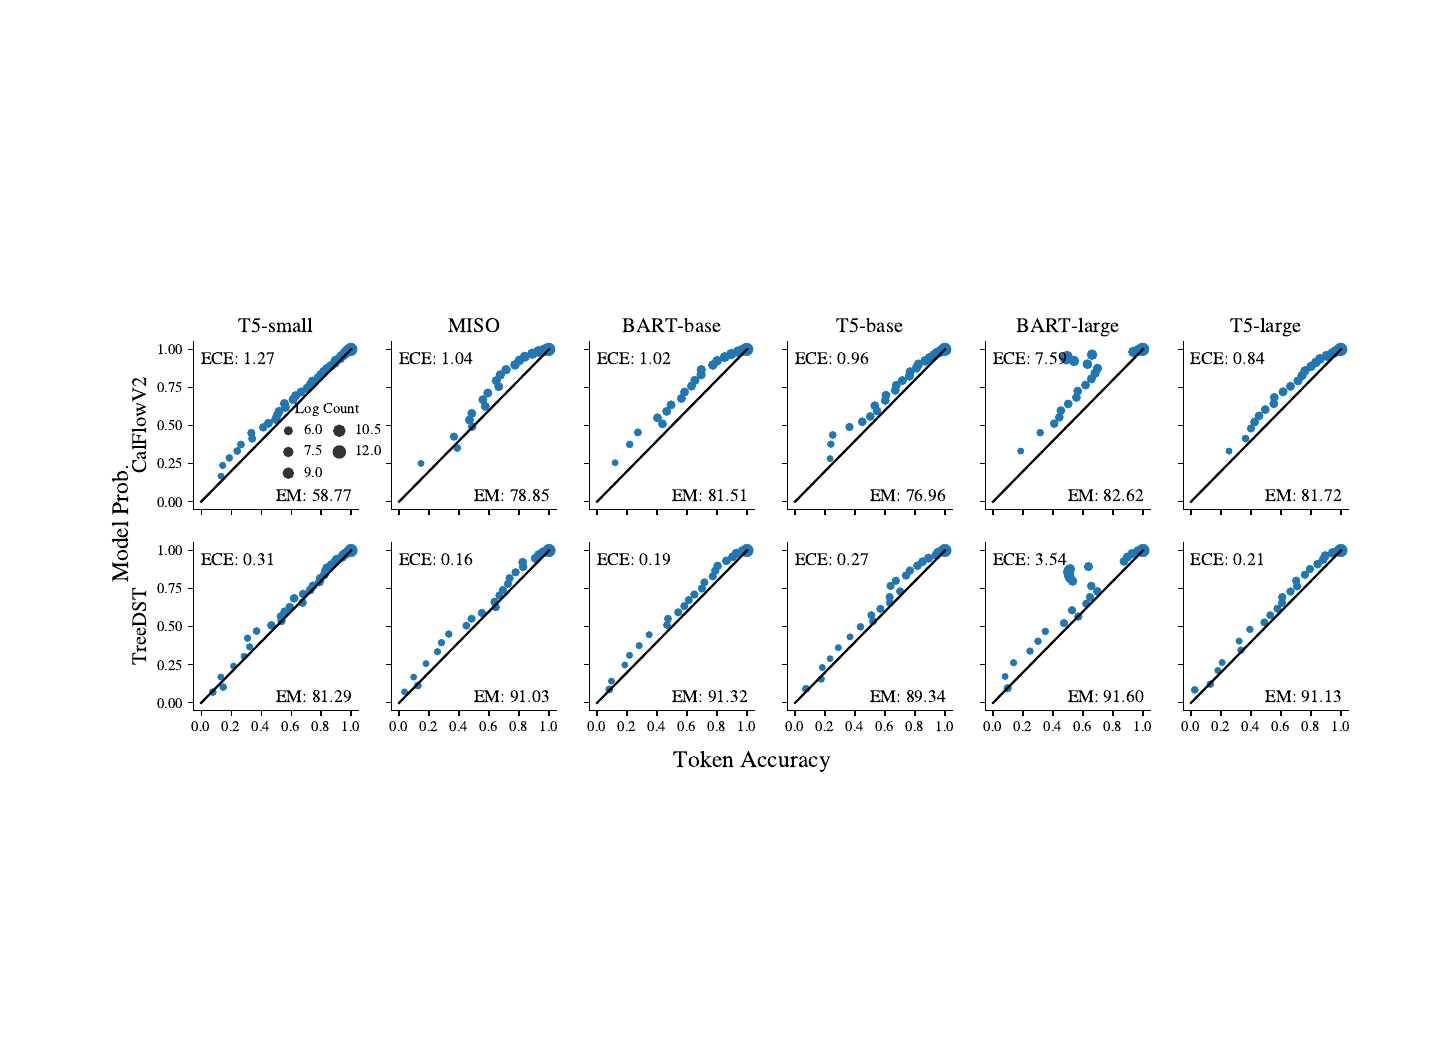
\includegraphics[width=3.363cm]{figures/img/hero_collage/tile_0.png}}};
\draw[black!35,line width=0.35pt] (0.070,-1.150) rectangle (3.433,-3.571);
\node[anchor=north west,text=ACMDarkBlue,font=\tiny\bfseries,inner sep=0] at (0.100,-3.601) {\href{https://arxiv.org/abs/2211.07443}{\adjustbox{max width=3.303cm}{Stengel-Eskin and Van Durme 2023}}};
\node[anchor=north west,text=black!60,font=\tiny,inner sep=0] at (0.100,-3.806) {\href{https://arxiv.org/abs/2211.07443}{Fig. 1, p.~6}};
\node[anchor=north west,inner sep=0] at (3.502,-1.150) {\href{https://arxiv.org/abs/2607.16799}{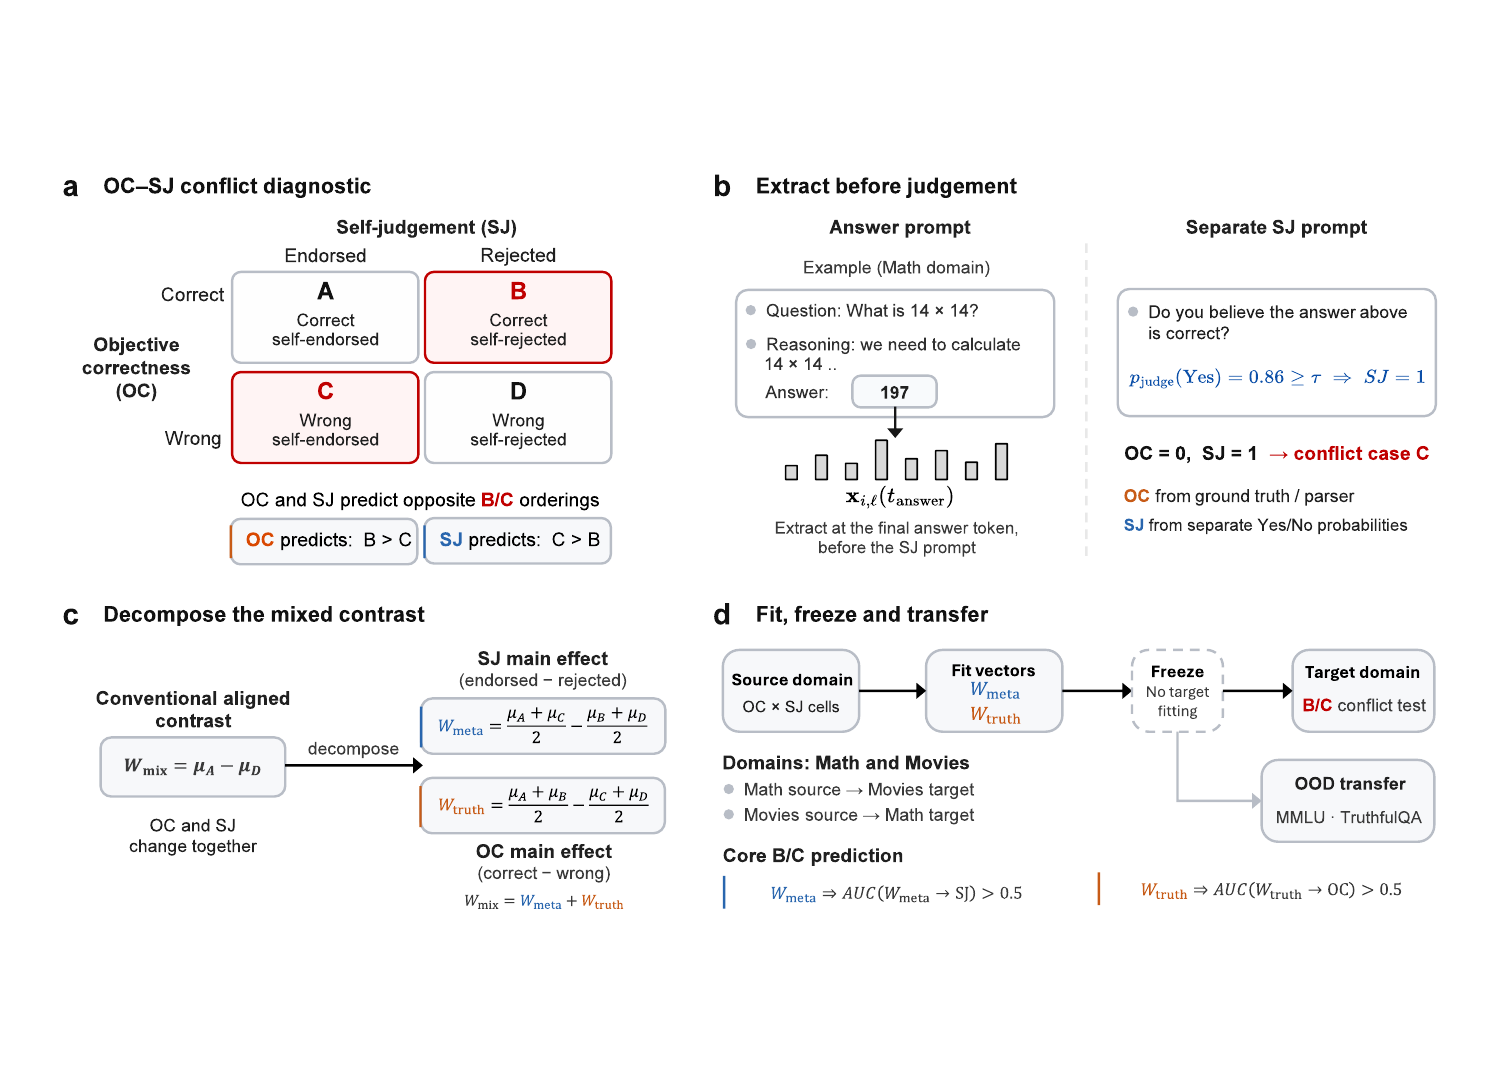
\includegraphics[width=3.363cm]{figures/img/hero_collage/tile_1.png}}};
\draw[black!35,line width=0.35pt] (3.502,-1.150) rectangle (6.865,-3.571);
\node[anchor=north west,text=ACMDarkBlue,font=\tiny\bfseries,inner sep=0] at (3.532,-3.601) {\href{https://arxiv.org/abs/2607.16799}{\adjustbox{max width=3.303cm}{Lu 2026}}};
\node[anchor=north west,text=black!60,font=\tiny,inner sep=0] at (3.532,-3.806) {\href{https://arxiv.org/abs/2607.16799}{Fig. 1, p.~2}};
\node[anchor=north west,inner sep=0] at (6.935,-1.150) {\href{https://arxiv.org/abs/2606.17234}{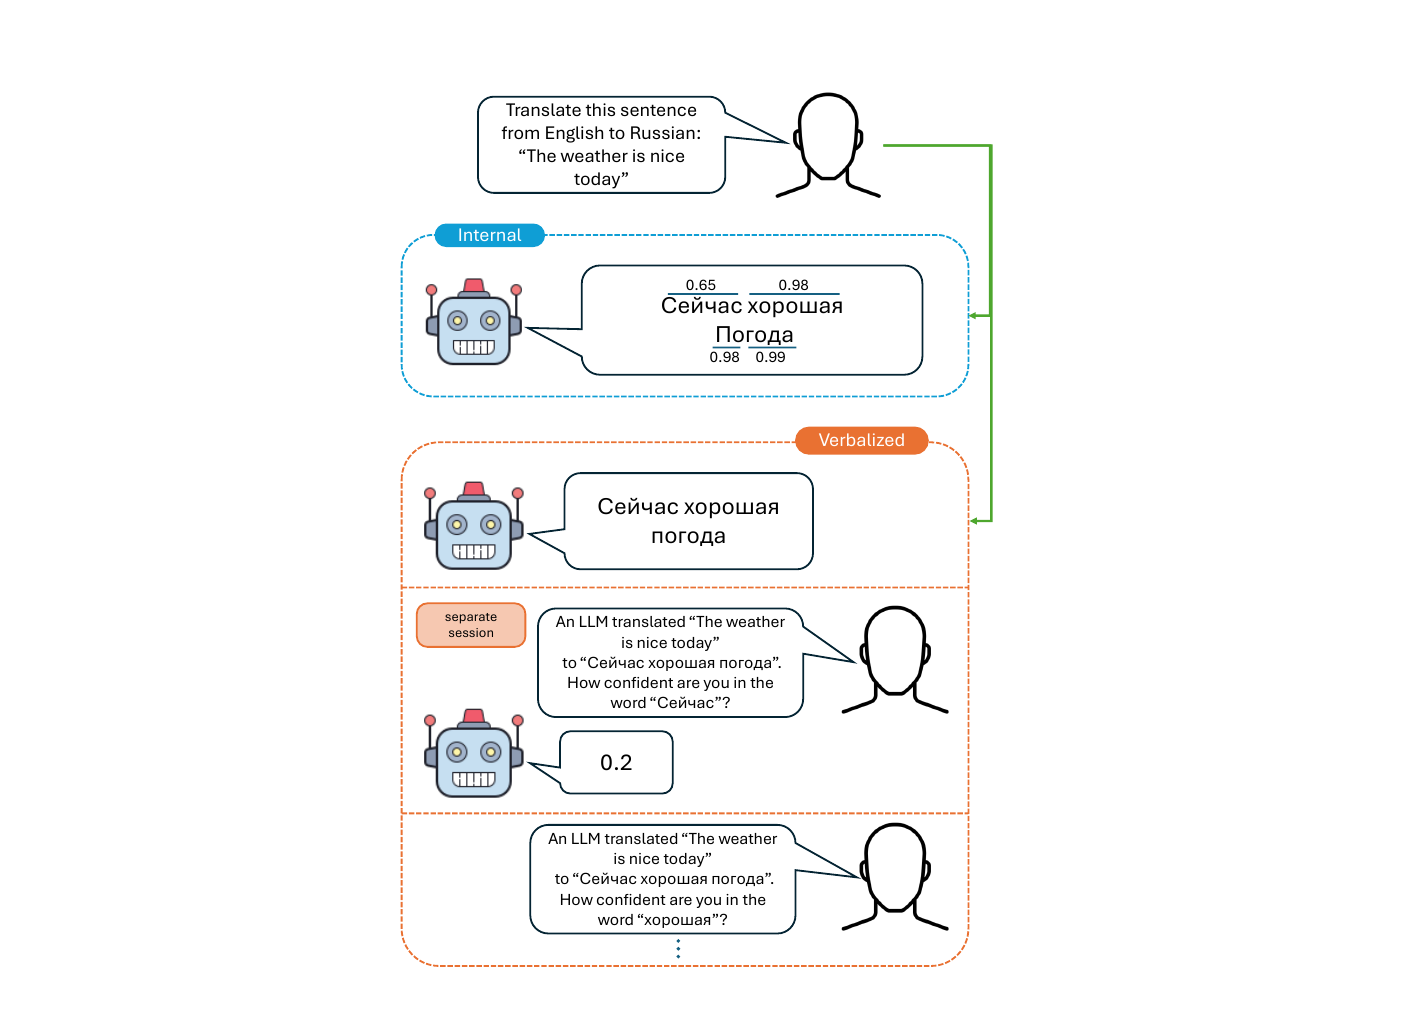
\includegraphics[width=3.363cm]{figures/img/hero_collage/tile_2.png}}};
\draw[black!35,line width=0.35pt] (6.935,-1.150) rectangle (10.298,-3.571);
\node[anchor=north west,text=ACMDarkBlue,font=\tiny\bfseries,inner sep=0] at (6.965,-3.601) {\href{https://arxiv.org/abs/2606.17234}{\adjustbox{max width=3.303cm}{Marashian et al. 2026}}};
\node[anchor=north west,text=black!60,font=\tiny,inner sep=0] at (6.965,-3.806) {\href{https://arxiv.org/abs/2606.17234}{Fig. 1, p.~1}};
\node[anchor=north west,inner sep=0] at (10.367,-1.150) {\href{https://arxiv.org/abs/2505.09427}{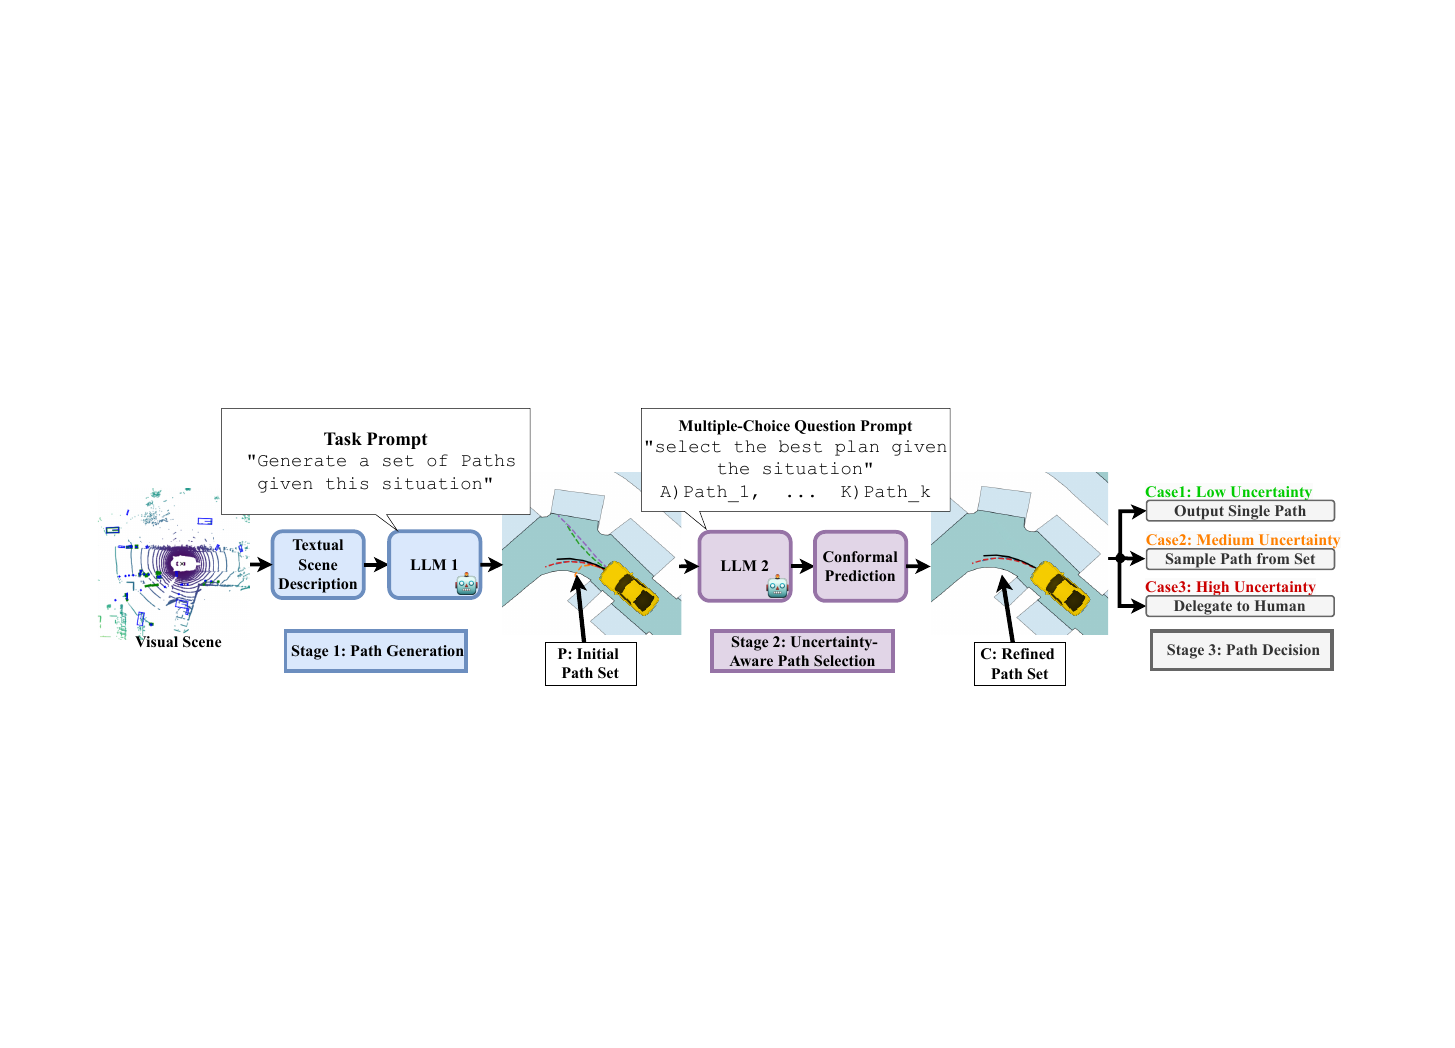
\includegraphics[width=3.363cm]{figures/img/hero_collage/tile_3.png}}};
\draw[black!35,line width=0.35pt] (10.367,-1.150) rectangle (13.730,-3.571);
\node[anchor=north west,text=ACMDarkBlue,font=\tiny\bfseries,inner sep=0] at (10.397,-3.601) {\href{https://arxiv.org/abs/2505.09427}{\adjustbox{max width=3.303cm}{Doula et al. 2025}}};
\node[anchor=north west,text=black!60,font=\tiny,inner sep=0] at (10.397,-3.806) {\href{https://arxiv.org/abs/2505.09427}{Fig. 1, p.~3}};
\fill[c7C5471] (0,-4.061) rectangle (13.800,-4.561);
\node[anchor=west,text=white,font=\footnotesize\bfseries,inner sep=0] at (0.14,-4.311) {Trained into the model: a calibration term in the training loss or reward (S4)};
\node[anchor=north west,inner sep=0] at (1.786,-4.631) {\href{https://arxiv.org/abs/2607.01612}{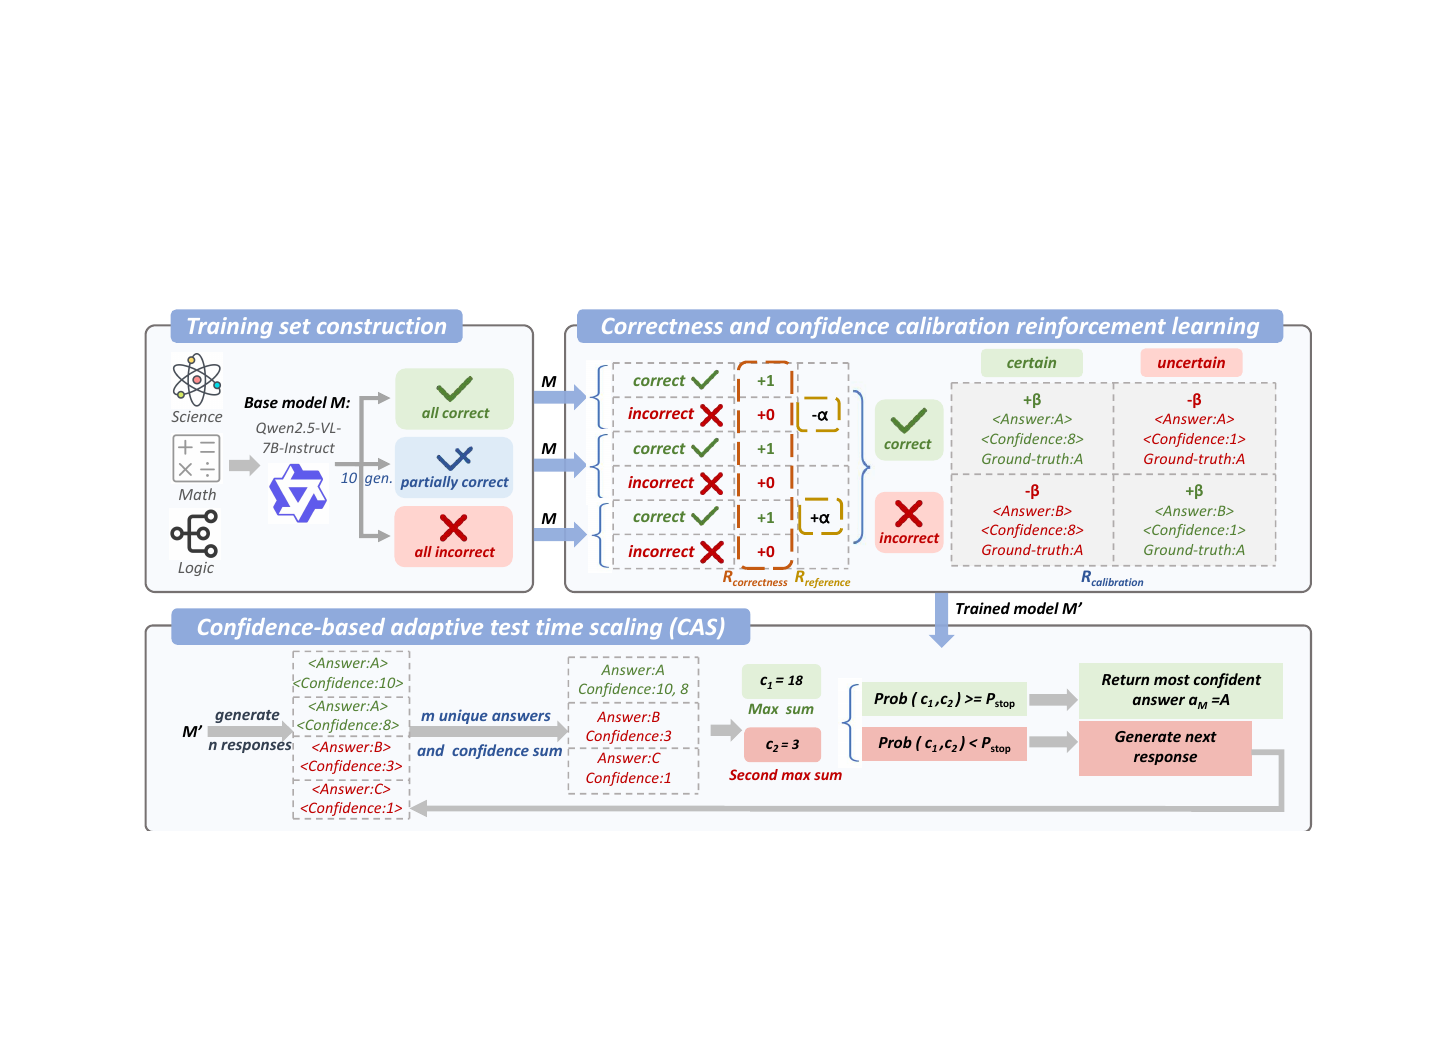
\includegraphics[width=3.363cm]{figures/img/hero_collage/tile_4.png}}};
\draw[black!35,line width=0.35pt] (1.786,-4.631) rectangle (5.149,-7.052);
\node[anchor=north west,text=ACMDarkBlue,font=\tiny\bfseries,inner sep=0] at (1.816,-7.082) {\href{https://arxiv.org/abs/2607.01612}{\adjustbox{max width=3.303cm}{Yang et al. 2026b}}};
\node[anchor=north west,text=black!60,font=\tiny,inner sep=0] at (1.816,-7.287) {\href{https://arxiv.org/abs/2607.01612}{Fig. 1, p.~3}};
\node[anchor=north west,inner sep=0] at (5.219,-4.631) {\href{https://arxiv.org/abs/2604.05306}{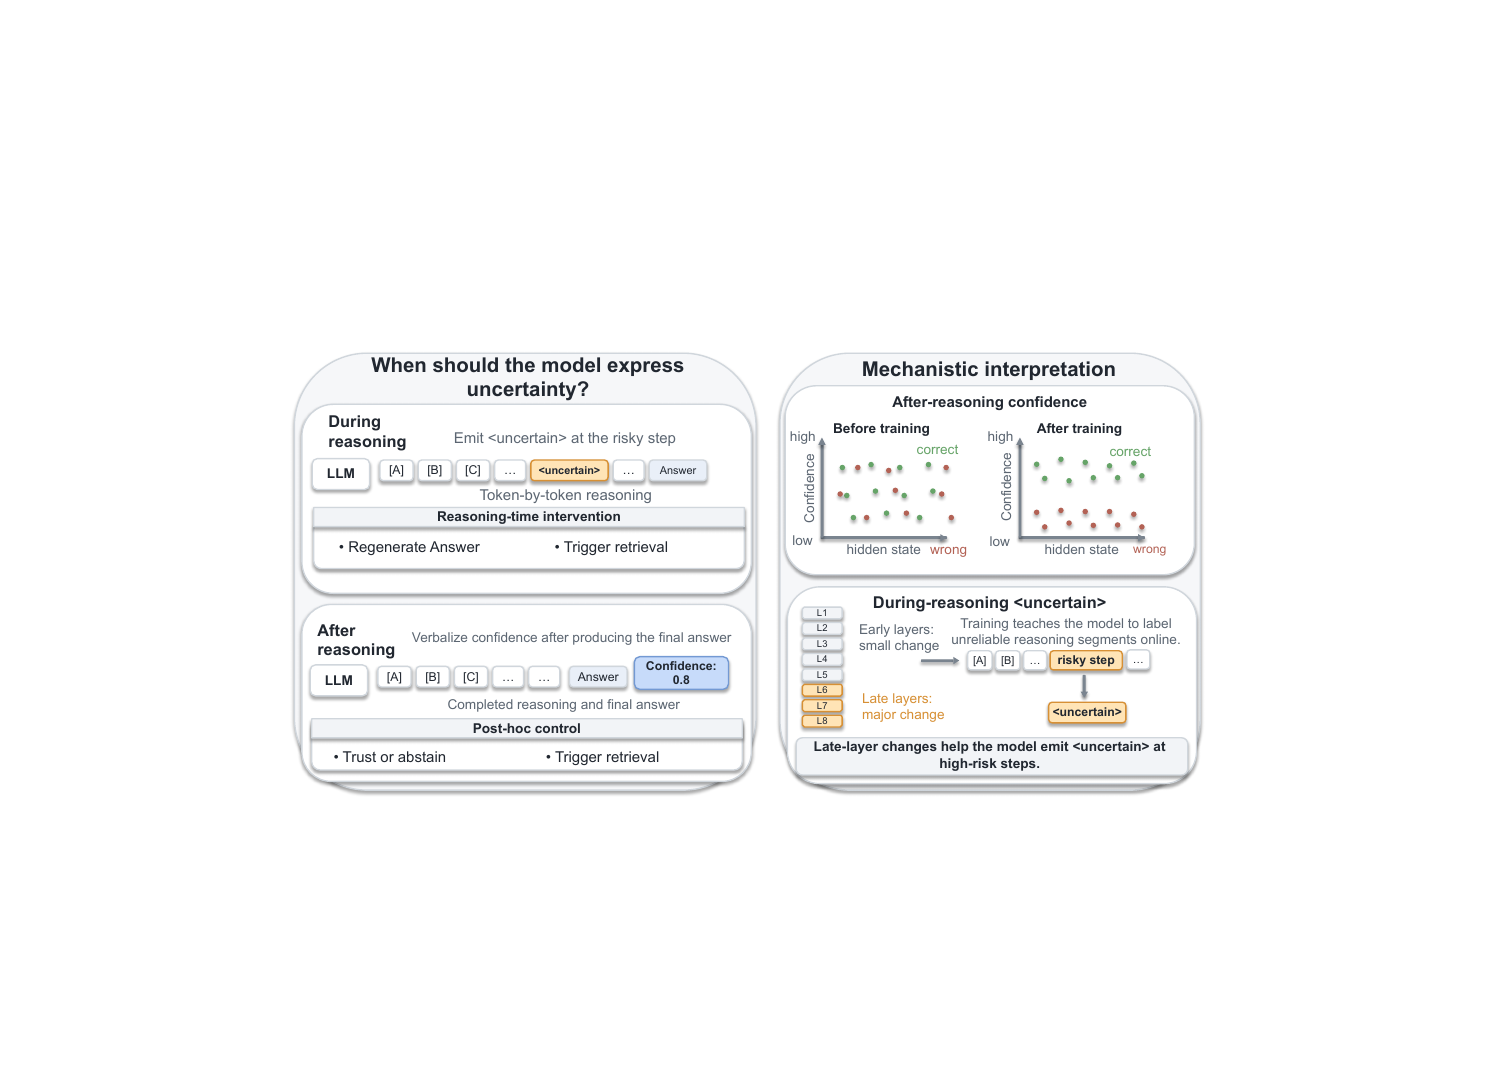
\includegraphics[width=3.363cm]{figures/img/hero_collage/tile_5.png}}};
\draw[black!35,line width=0.35pt] (5.219,-4.631) rectangle (8.581,-7.052);
\node[anchor=north west,text=ACMDarkBlue,font=\tiny\bfseries,inner sep=0] at (5.249,-7.082) {\href{https://arxiv.org/abs/2604.05306}{\adjustbox{max width=3.303cm}{Guo et al. 2026}}};
\node[anchor=north west,text=black!60,font=\tiny,inner sep=0] at (5.249,-7.287) {\href{https://arxiv.org/abs/2604.05306}{Fig. 1, p.~2}};
\node[anchor=north west,inner sep=0] at (8.651,-4.631) {\href{https://arxiv.org/abs/2604.22779}{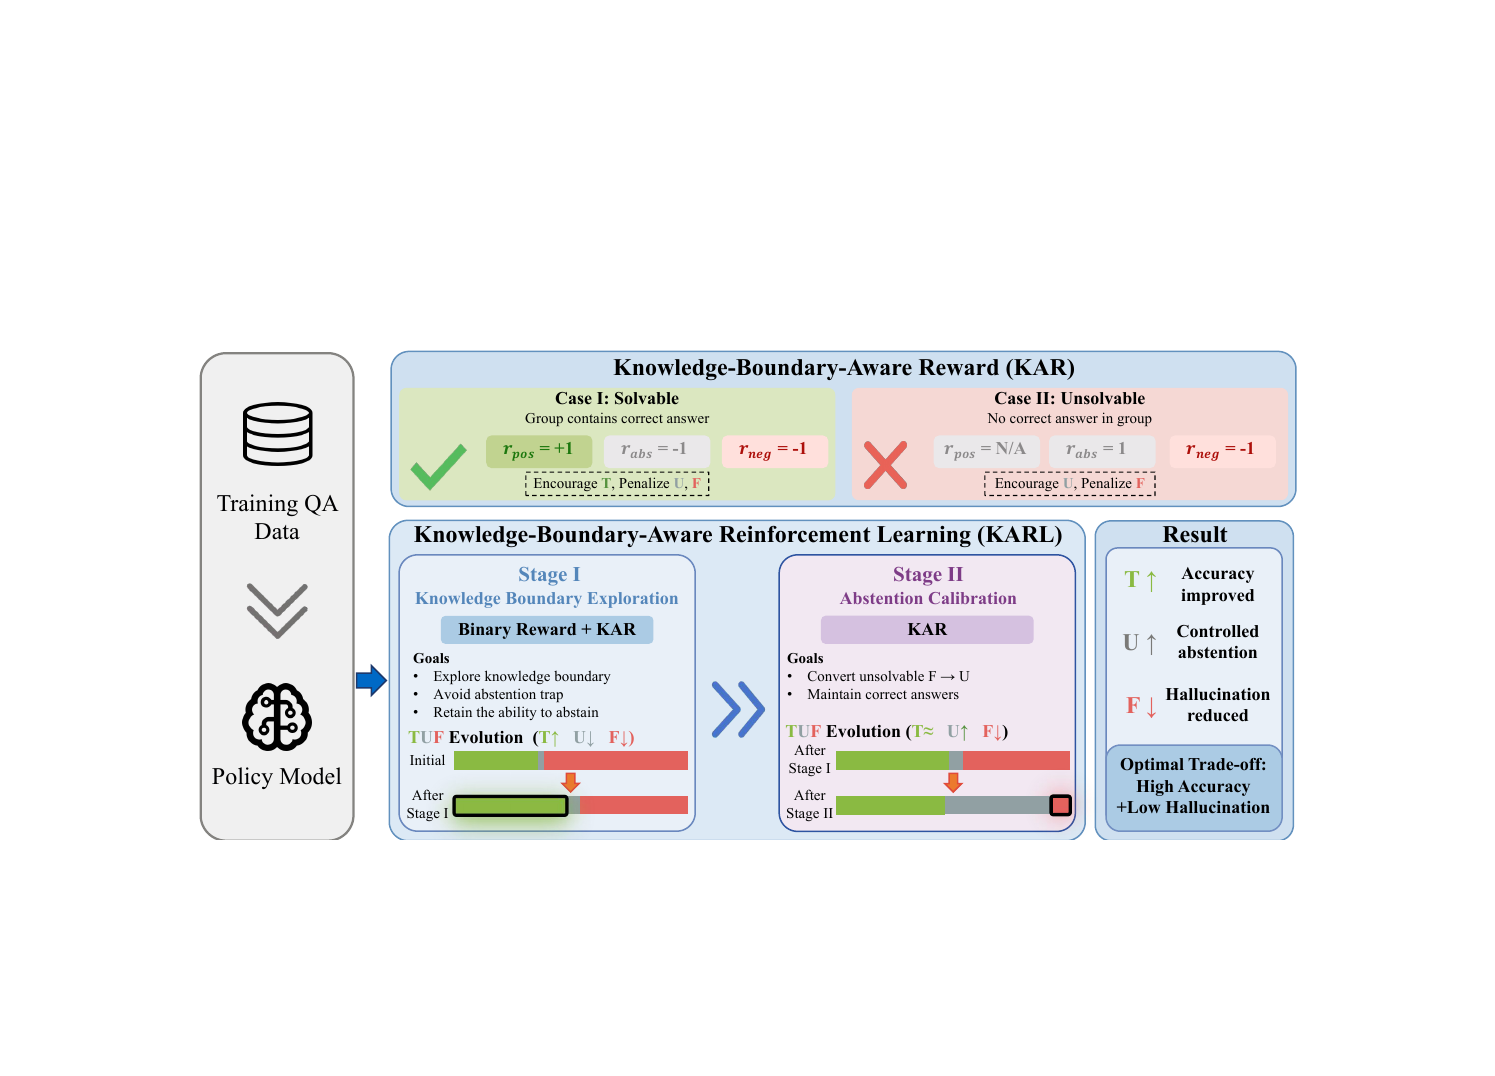
\includegraphics[width=3.363cm]{figures/img/hero_collage/tile_6.png}}};
\draw[black!35,line width=0.35pt] (8.651,-4.631) rectangle (12.014,-7.052);
\node[anchor=north west,text=ACMDarkBlue,font=\tiny\bfseries,inner sep=0] at (8.681,-7.082) {\href{https://arxiv.org/abs/2604.22779}{\adjustbox{max width=3.303cm}{Gao et al. 2026}}};
\node[anchor=north west,text=black!60,font=\tiny,inner sep=0] at (8.681,-7.287) {\href{https://arxiv.org/abs/2604.22779}{Fig. 4, p.~4}};
\end{tikzpicture}}
\caption{\textbf{Confidence estimated after the fact, and confidence trained into the model.} Panels are drawn from Figures~\ref{fig:method_gallery} and~\ref{fig:results_gallery} under the same licence rule: one per stage for S0, S1, S2, S3, and one per training family for S4 (T1, T3, T4; T2, T5 not shown). Each label links to the paper; Table~\ref{tab:panel_provenance} gives the figure, page and licence.}
\Description{A labelled grid of images, each a hyperlink annotated with its system name and source figure number.}
\label{fig:hero_collage}
\end{figure*}
